\section{Protótipos para a interface da aplicação}

Um dos processos de desenvolvimento de uma Aplicação Web é a criação de protótipos. Este processo tem como objetivo demonstrar de que forma o utilizador interage com a aplicação e ajuda a tomar decisões antes da implementação da aplicação. Desta forma há um maior entendimento entre o utilizador e a equipa de desenvolvimento e aumenta a usabilidade da aplicação por parte do utilizador, uma vez que são garantidas as seguintes habilidades:

\begin{description}
	\item[Fácil apendizagem] A utilização da aplicação requer pouco treino
	\item[Fácil de memorizar] O utilizador lembra-se de como utilizar a interface depois algum tempo
	\item[Maximizar a produtividade] A realização de uma tarefa é feita de forma rápida e eficiente
	\item[Minimizar a taxa de erros] A aplicação avisa o utlizador, caso existam erros e ajuda na correção dos mesmos
	\item[Maximizar a satisfação] A aplicação transmite confiança e segurança ao utilizador
\end{description}

 \subsection{Primeiros protótipos}

Durante a produção dos primeiros protótipos, teve-se como objetivo identificar de que formas as várias funcionalidades do sistemas iriam estar presentes na aplicação, sem haver preocupações com questões estéticas.Este protótipos são fundamentais, uma vez que demonstrem alguns dos cenários mais complexos e ajuda a compreensão de fluxos ou processos.
Este protótipos foram desenvolvidos usando a aplicação \href{http://balsamiq.com/products/mockups/}{\emph{Balsamiq Mockups}}(Figura ~\ref{fig: balsamiq}).\\

 \begin{figure}[htbp]
        \centering
        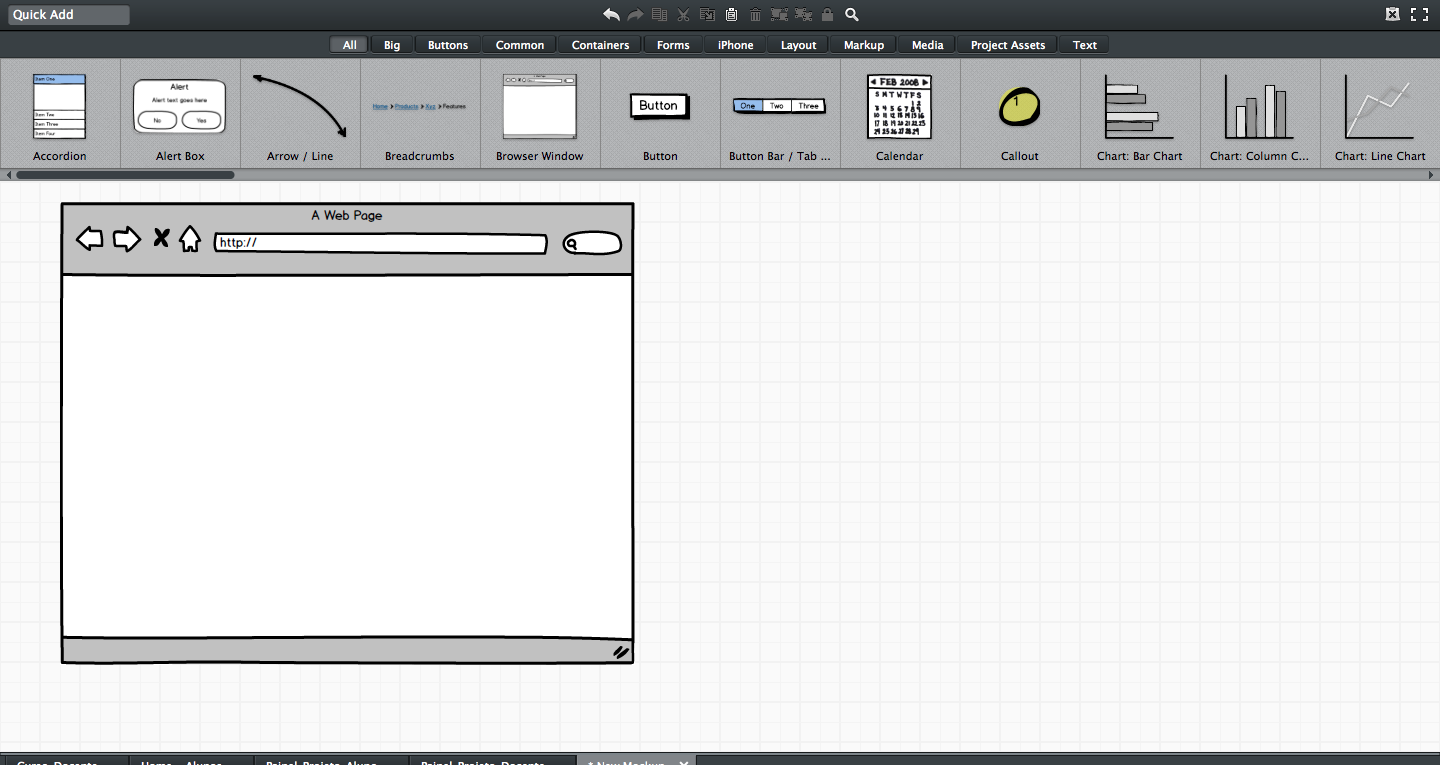
\includegraphics[width=1\textwidth]{images/prototipos/mockups/balsamiq.png}
         \caption{\emph{Balsamiq Mockups}}
         \label{fig: balsamiq}
\end{figure}

Sobre os protótipos desenvolvidos, teve-se como preocupação a simplicidade da página, a quantidade de informação e o tempo de navegação, isto é a quantidade de ações que um utilizador tem que fazer para passar de uma página para outra.\\
Começando pela página inicial (Figura ~\ref{fig: home}) está mostra as várias funcionalidades da aplicação, fazendo a distinção entre alunos e docentes.A partir da página inicial o utilizador pode fazer efetuar registo, login ou procura projetos públicos. \\

\begin{figure}[htbp]
        \centering
        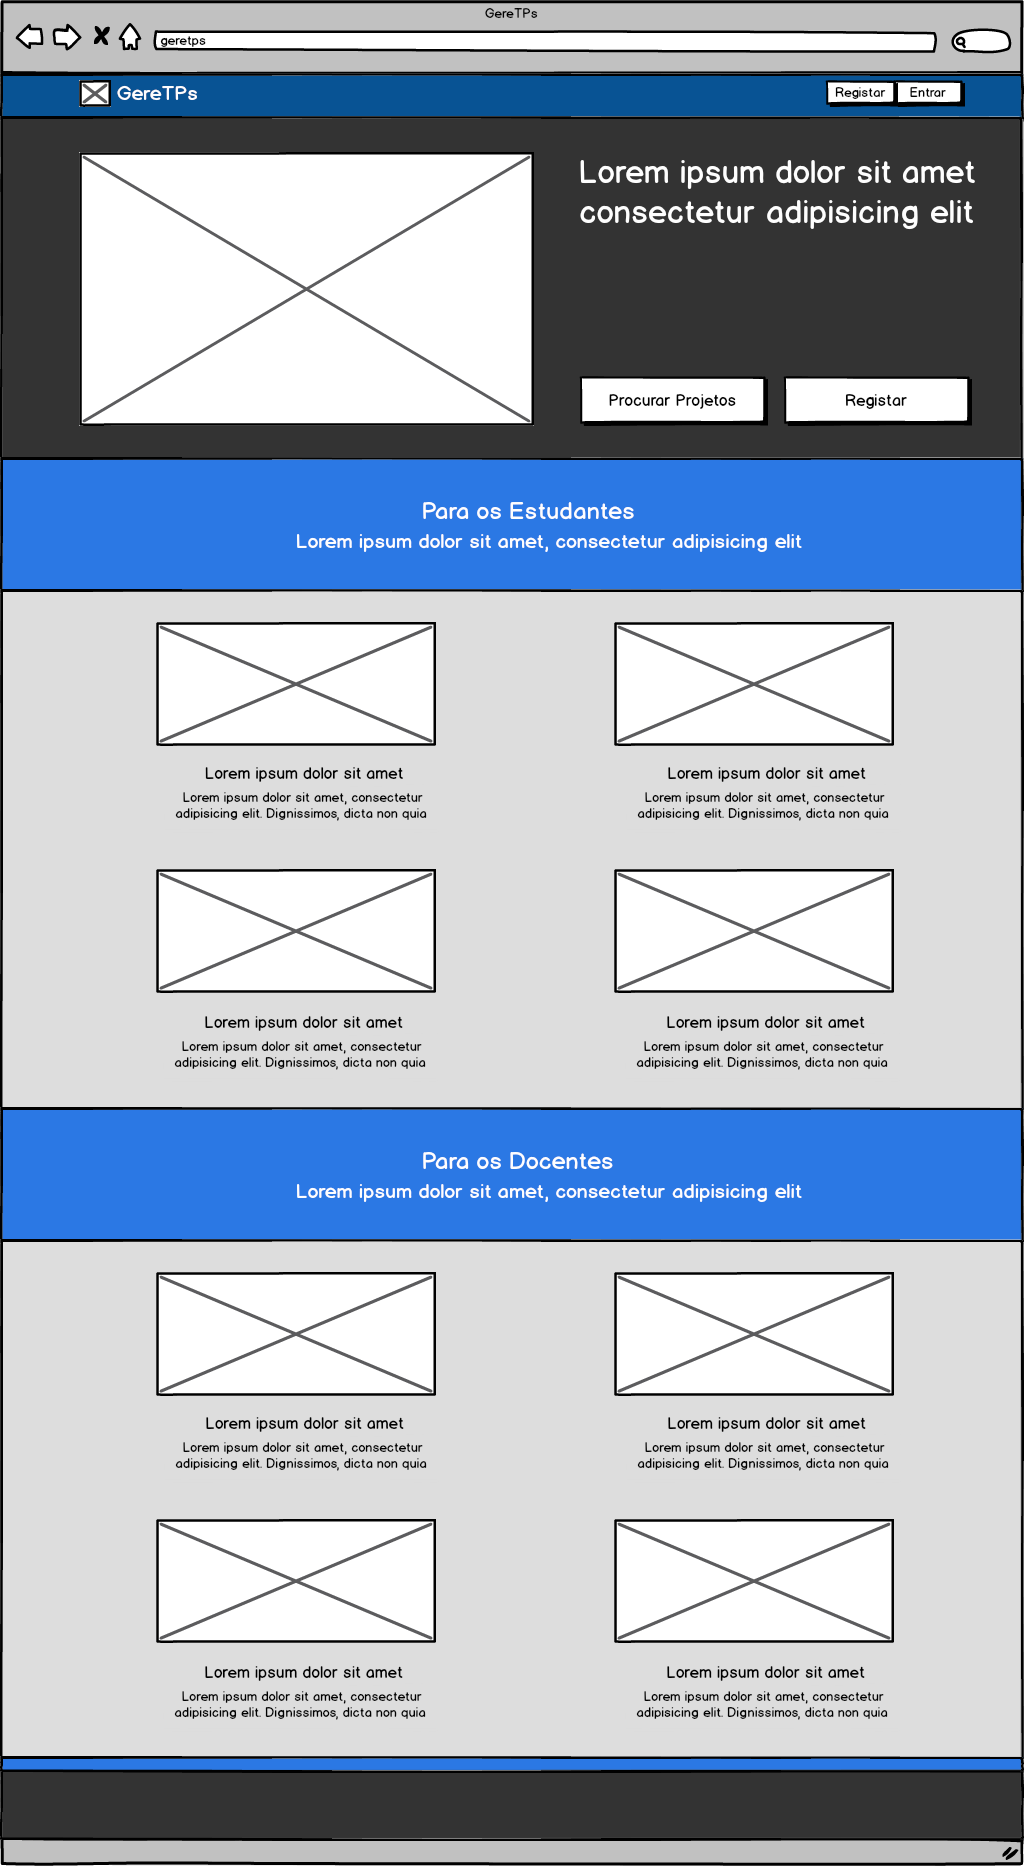
\includegraphics[width=1\textwidth]{images/prototipos/mockups/home.png}
         \caption{Página inicial}
         \label{fig: home}
\end{figure}

No painel de uma disciplina(Figura ~\ref{fig: cursodocente}), um docente pode ter acesso aos últimos acontecimentos dentro das disciplina, sabendo quando aconteceram submissões nos projetos desta, assim como alterações da mesma.Também existem informações sobre os projetos criados na disciplina, no qual são apresentadas informações sobre o nome do projeto, número de fases, estado e número de entregas até ao momento. Também é possível adicionar professores de forma direta sem que haja a necessidade de abrir formulários adicionais e fazer gestão de turnos. Caso contrário apenas poderá ver o estado dos turnos e quais são os docentes da disciplina.\\

\begin{figure}[htbp]
        \centering
        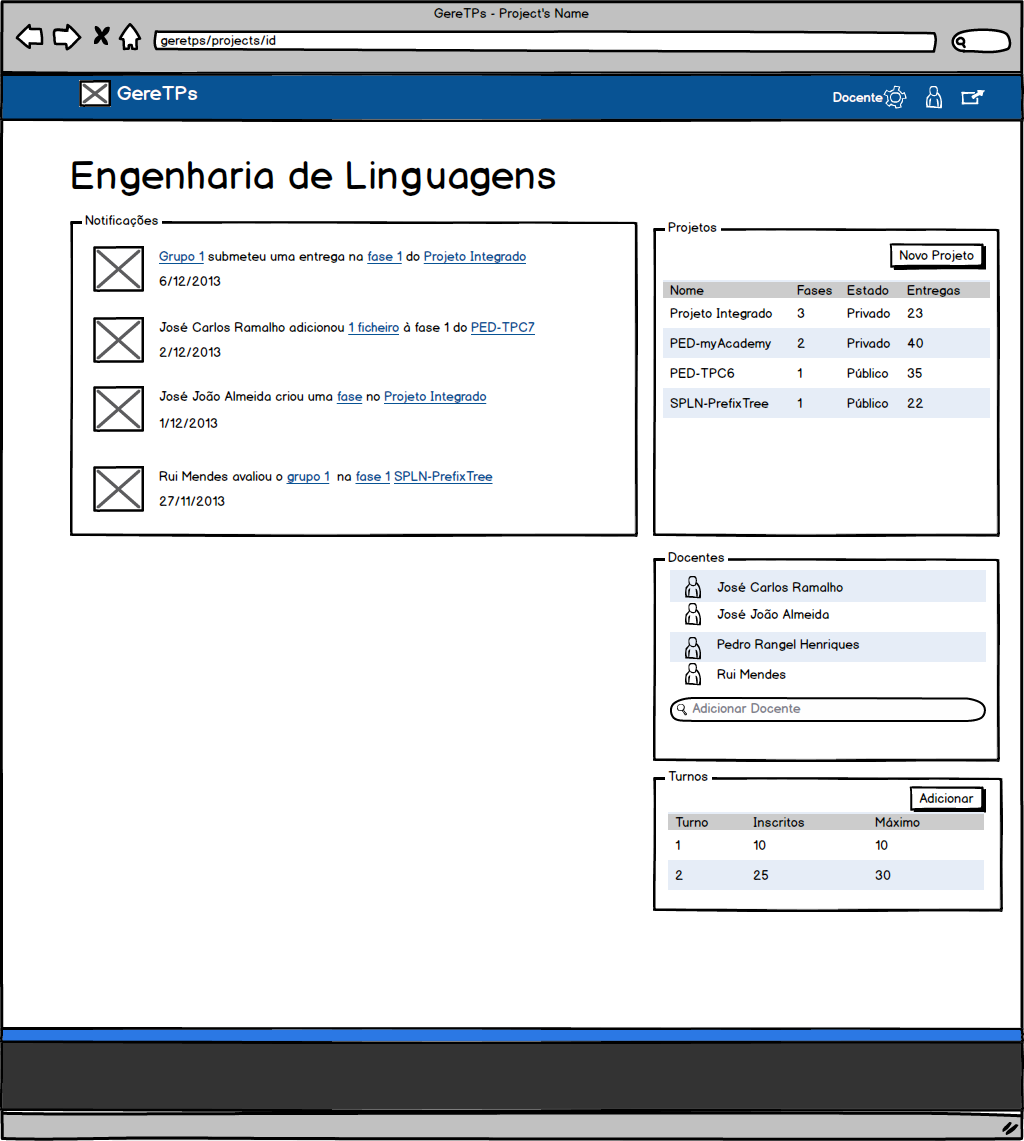
\includegraphics[width=1\textwidth]{images/prototipos/mockups/cursodocente.png}
         \caption{Painel de projeto de um aluno}
         \label{fig: cursodocente}
\end{figure}

Na painel de pesquisa de projetos(Figura ~\ref{fig: projetospublicos}), todos os utilizadores tem acesso aos projetos públicos. Nesta página o utilizador pode filtrar uma pesquisa de forma a que o processo seja mais rápido. Os resultados de uma pesquisa são apresentados sob forma de blocos, desta forma, garante-se um maior aproveitamento do espaço livre da página.\\

\begin{figure}[htbp]
        \centering
        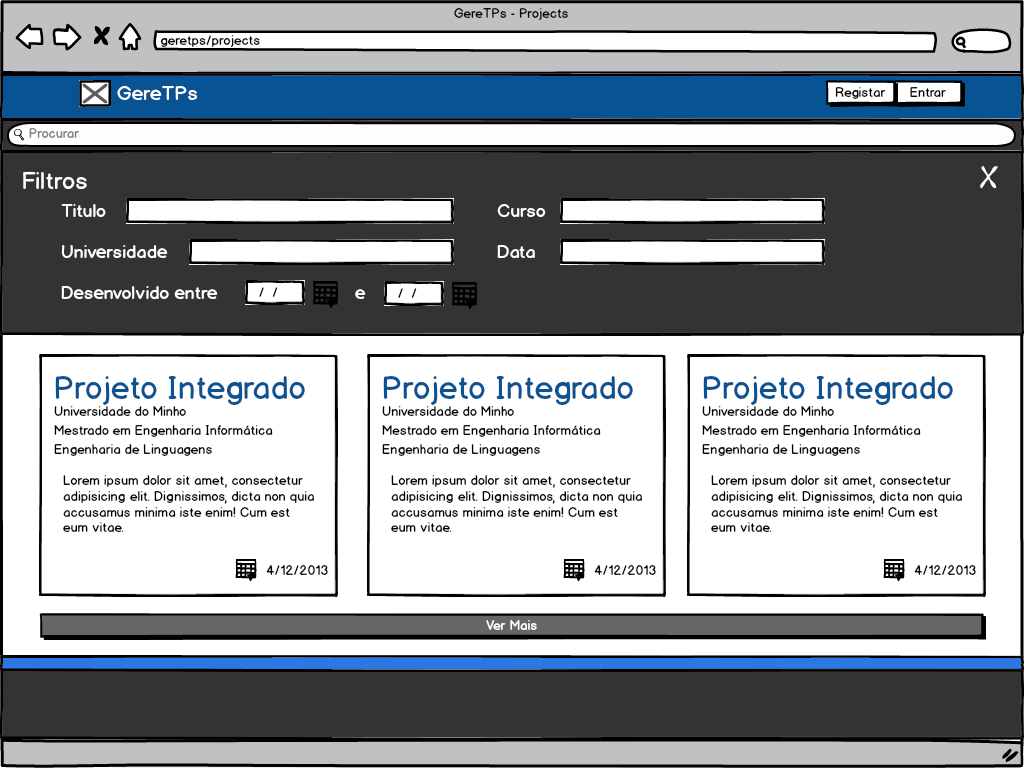
\includegraphics[width=1\textwidth]{images/prototipos/mockups/Projetos.png}
         \caption{Listagem dos projetos públicos}
         \label{fig: projetospublicos}
\end{figure}

Quando dentro do painel de um projeto, um docente pode:

\begin{itemize}
        \item Alterar informações do projeto
	\item Adicionar um enunciado, tal como outros ficheiros
	\item Gerir os grupos criados dentro do projeto
	\item Gerir as fases do projeto
	\item Consultar as submissões feitas até ao momento
        \item Adicionar/Remover testes
\end{itemize}
tal como se pode ver na Figura ~\ref{fig: painelprojetodocente}.\\

\begin{figure}[htbp]
        \centering
        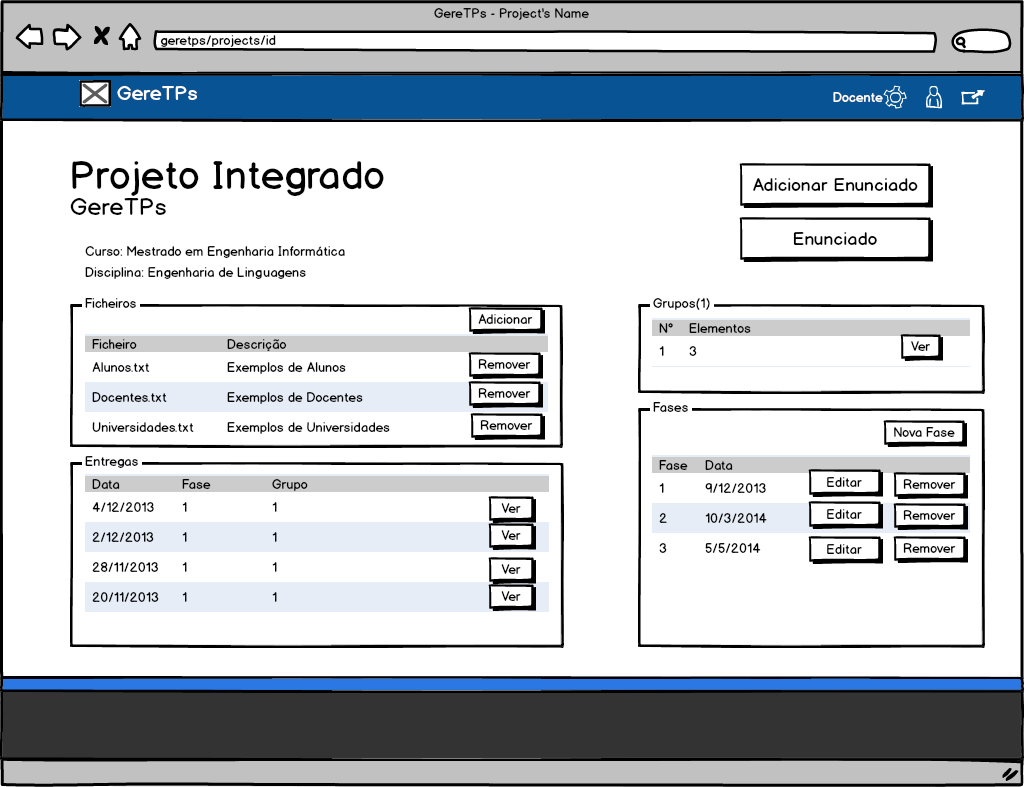
\includegraphics[width=1\textwidth]{images/prototipos/mockups/painelprojetodocente.png}
         \caption{Painel de projeto de um docente}
         \label{fig: painelprojetodocente}
\end{figure}

Um aluno pode consultar as informações dadas pelos os docente, consultar as entregas efetuadas pelo grupo, fazer a gestão do seu grupo e aceder a página de submissão de um projeto, como é possível ver na Figura ~\ref{fig: painelprojetoaluno}.\\

\begin{figure}[htbp]
        \centering
        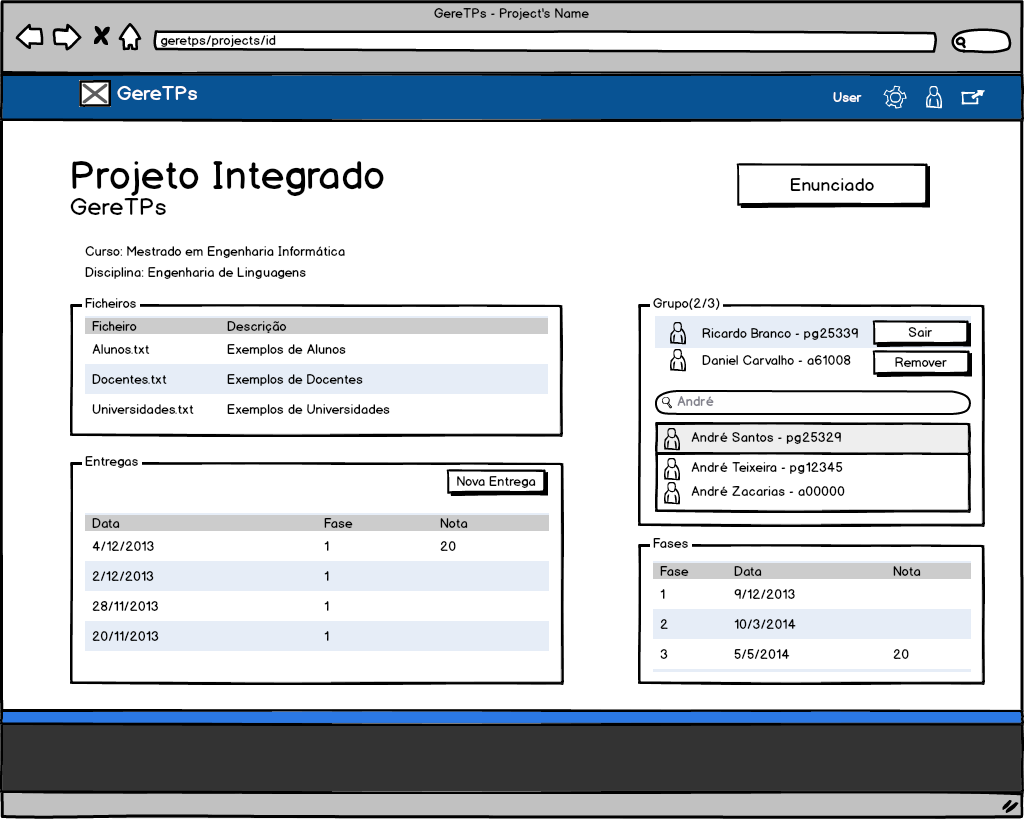
\includegraphics[width=1\textwidth]{images/prototipos/mockups/painelprojetoaluno.png}
         \caption{Painel de projeto de um aluno}
         \label{fig: painelprojetoaluno}
\end{figure}

Quando se visualiza um projeto, e de acordo com a Figura ~\ref{fig: projetoaluno}, pode-se aceder diretamente ao enunciado e relatório do projeto, ver e fazer \emph{Dowload} individual ou global(Ficheiro \emph{ZIP}) dos ficheiros submetidos, também é disponibilizado um resumo sob o trabalho feito, assim como a nota deste caso exista.Se for um docente responsável pela disciplina em que se enquadra o projeto a aceder à página, este pode fazer a avaliação do grupo, ou de cada membro individual e adicionar comentários sob a nota dada, tal como podemos ver na Figura ~\ref{fig: projetodocente}.\\

\begin{figure}[htbp]
        \centering
        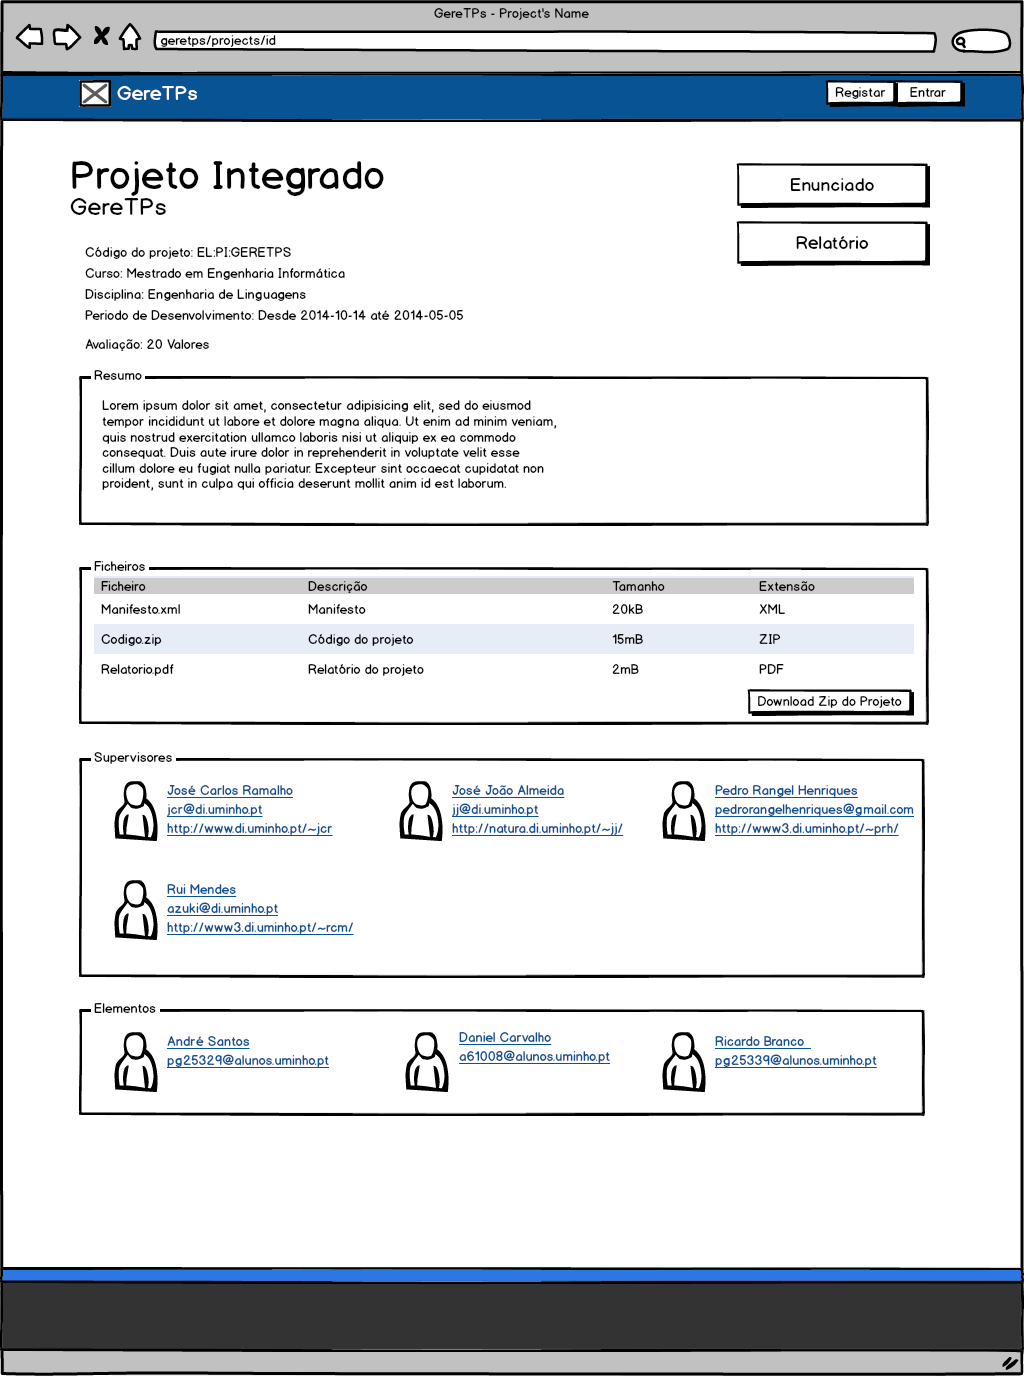
\includegraphics[width=1\textwidth]{images/prototipos/mockups/projetovisitante.png}
         \caption{Entrega vista por um visitante}
         \label{fig: projetoaluno}
\end{figure}

\begin{figure}[htbp]
        \centering
        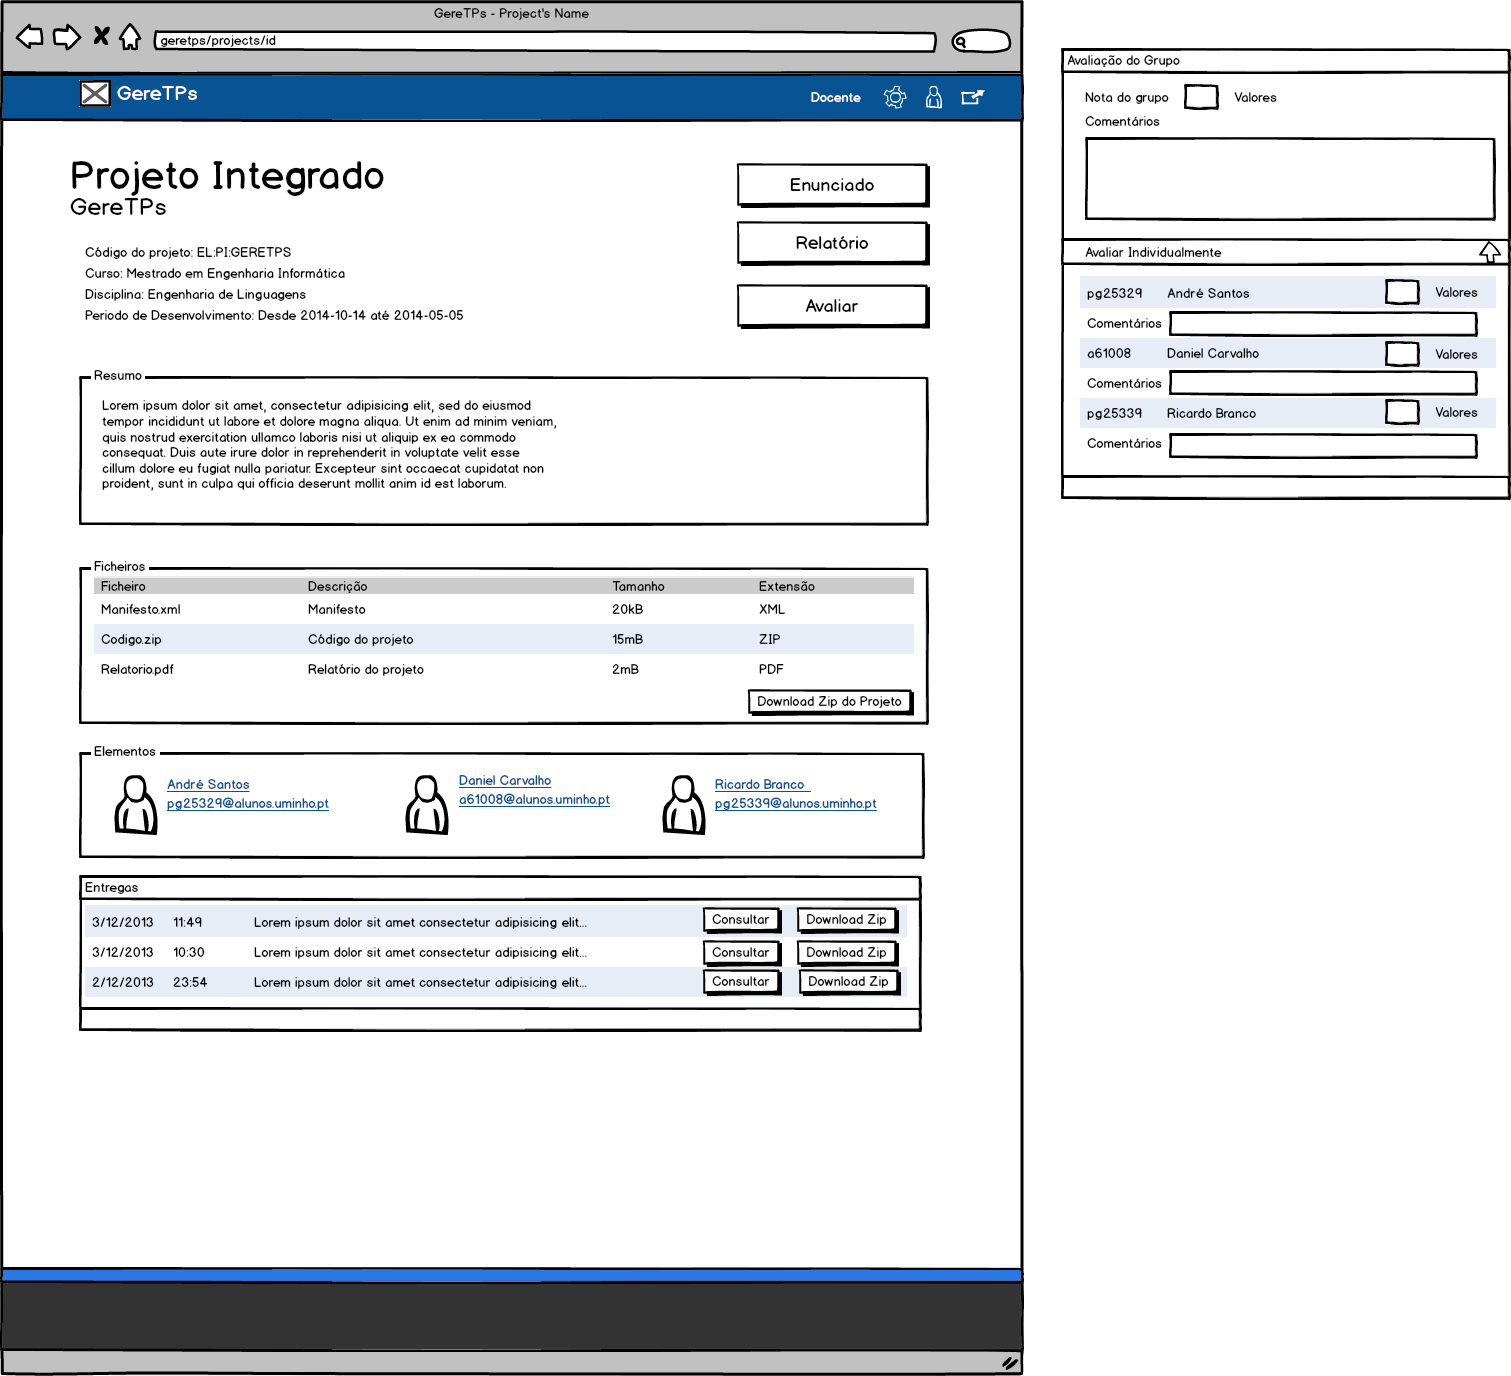
\includegraphics[width=1\textwidth]{images/prototipos/mockups/projetodocente.png}
         \caption{Entrega vista por um docente}
         \label{fig: projetodocente}
\end{figure}

\subsection{Protótipos fidedignos}
Para além dos primeiros protótipos, fizeram-se também protótipos fidedignos baseados nos anteriormente
citados de forma a aumentar o nível de detalhe, bem como aproximar a prototipagem o mais 
próximo possível do resultado final esperado. Assim sendo, segue-se na figura \ref{fig:prot_fid_home}
um exemplo da prototipagem fidedigna da página principal.
Com este tipo de protótipos espera-se aprimorar os detalhes, bem como os esquemas de cores,
arranjos gráficos, entre outros pormenores.
De notar que os protótipos fidedignos feitos neste projeto foram construídos diretamente a partir
da linguagem HTML.

\begin{figure}[H] 
  \centering
  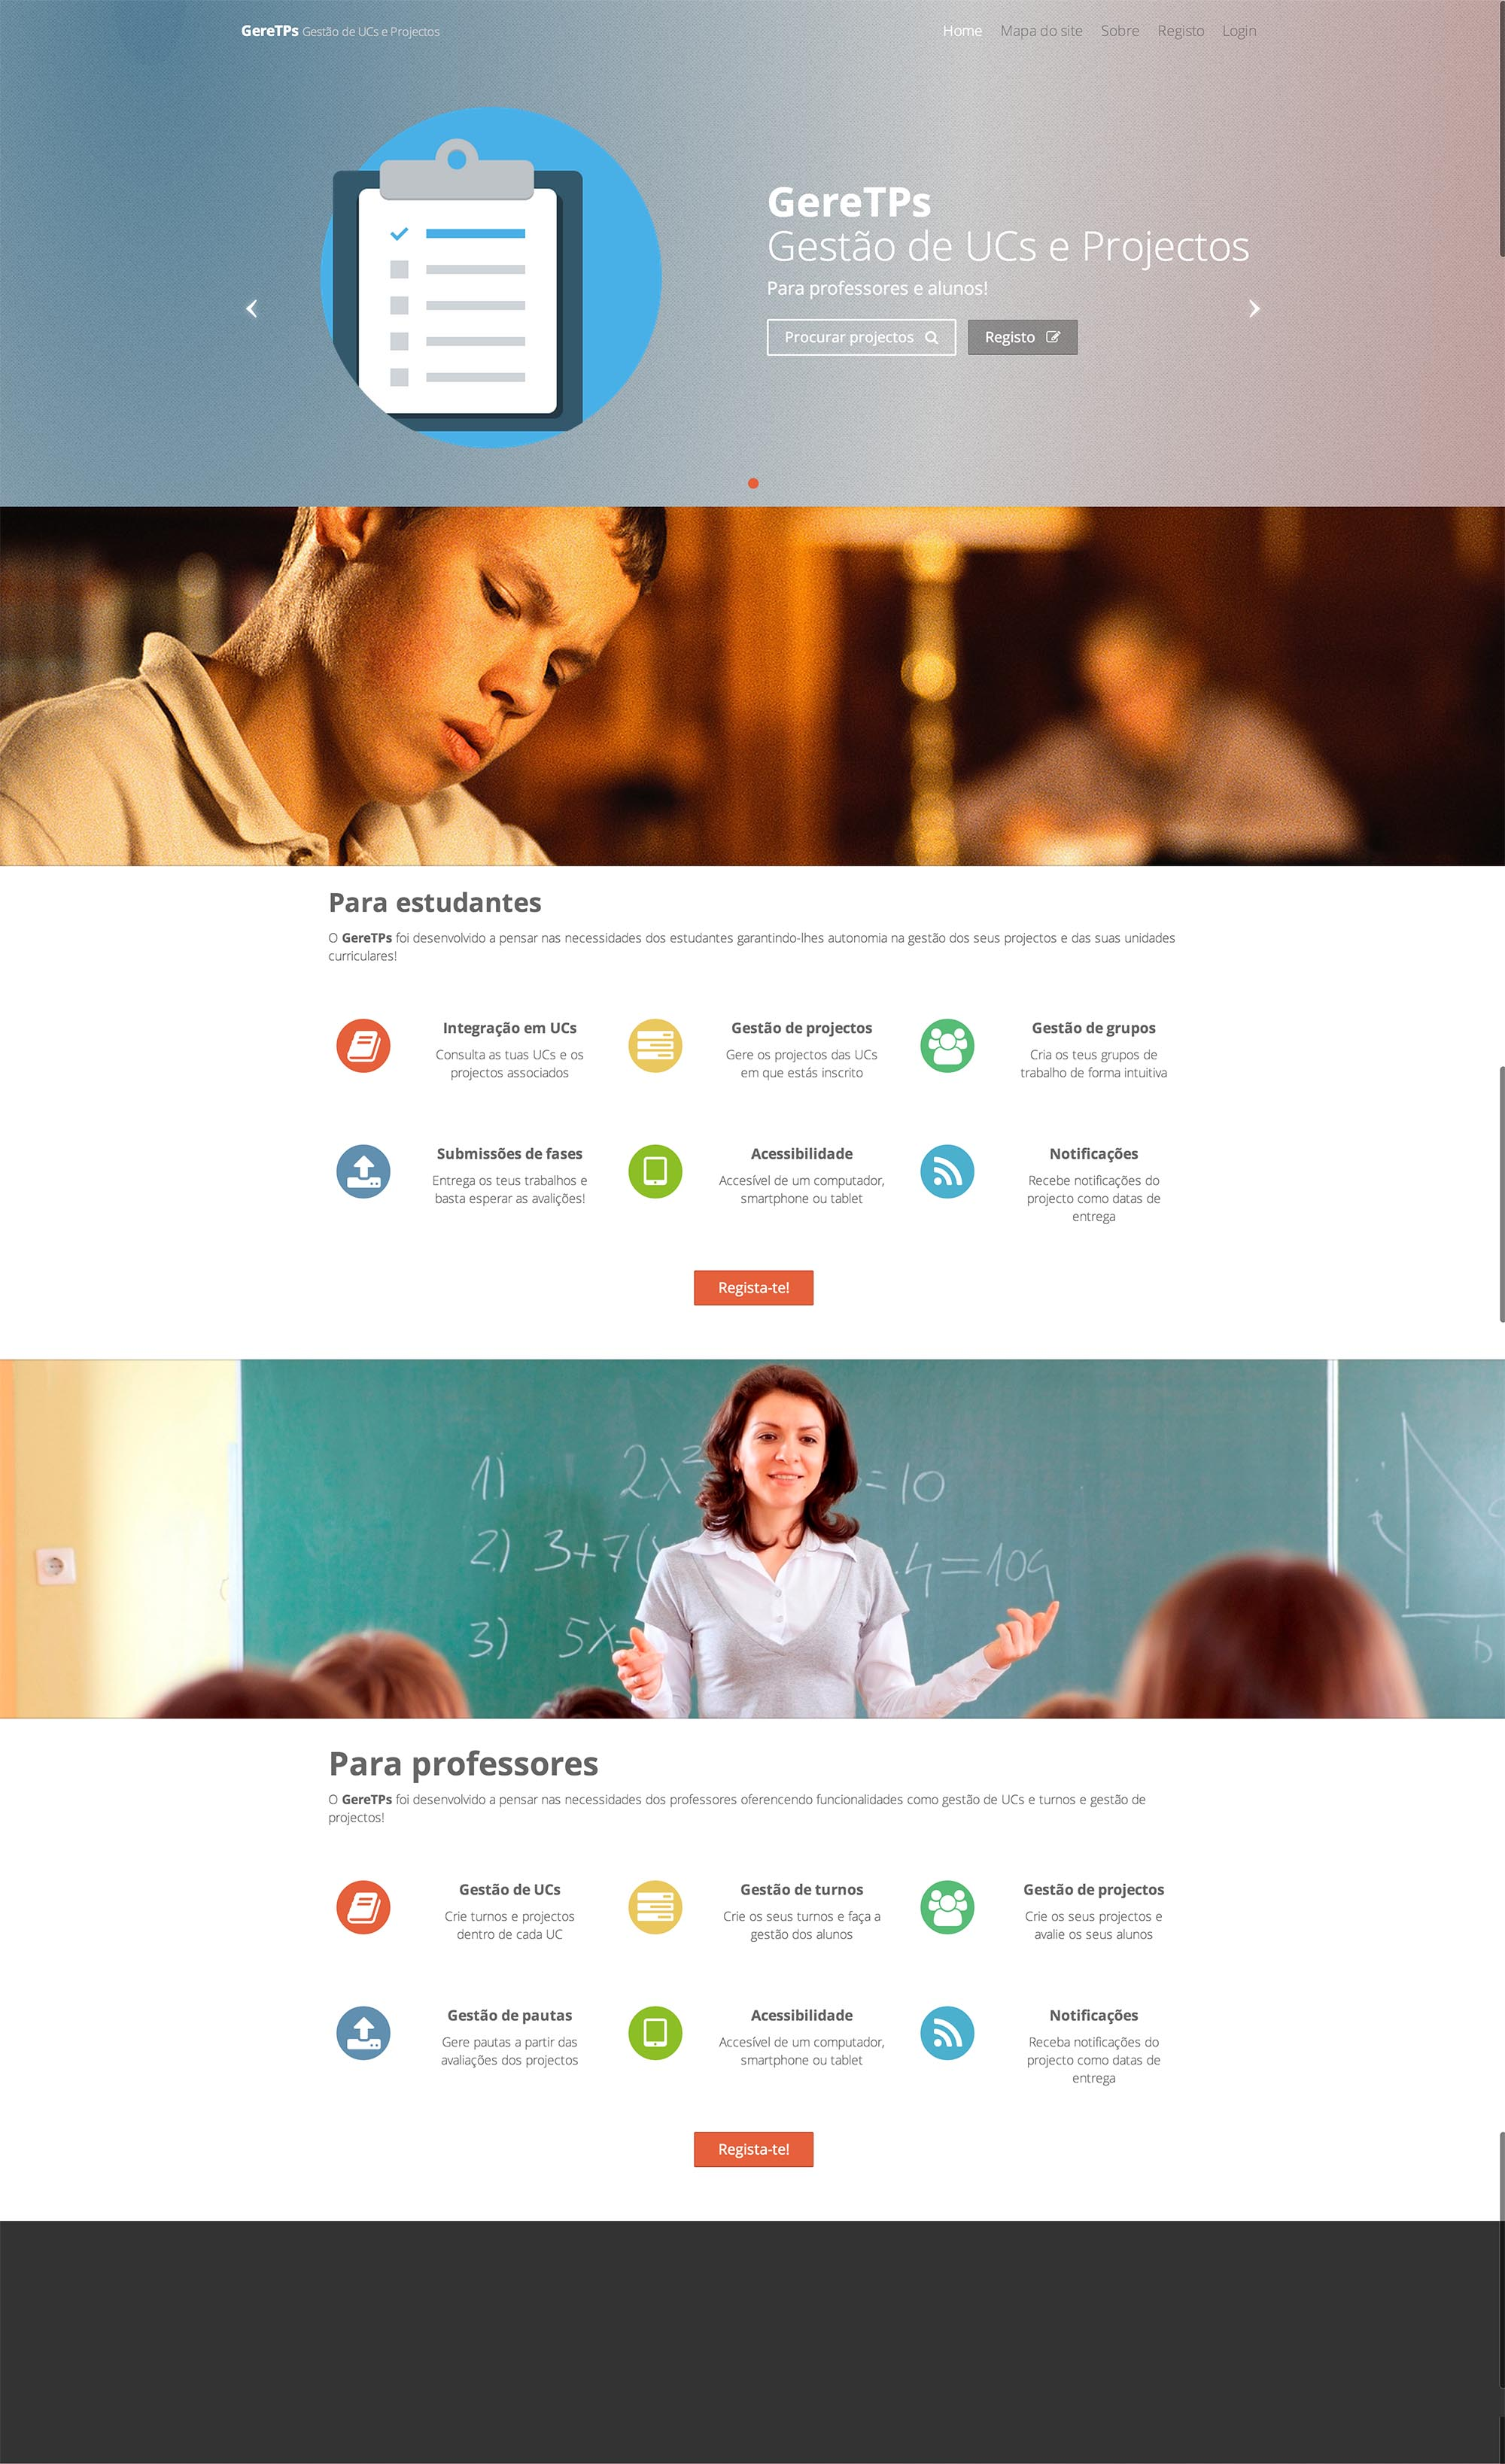
\includegraphics[width=0.8\textwidth,center]{images/prototipos/fidedigno_home.jpg}
  \caption{Protótipo fidedigno página inicial}
  \label{fig:prot_fid_home}
\end{figure}

\newpage

